%------------------------------------------------------------------------------
\begin{figure*}[t]
    \centering
    \resizebox{\textwidth}{!}{%
    \begin{tabular}{ccccccccc}
        {}&\multirow{2}{*}{Original}&\multirow{2}{*}{Raw Attention}&\multicolumn{2}{c}{Grad-CAM}&\multicolumn{2}{c}{Grad-CAM++}&\multicolumn{1}{c}{Score-CAM}\\
        {}&{}&{}&GAP&CLS&GAP&CLS&GAP&CLS\\
        {\rotatebox{90}{\small Waffle Iron}}&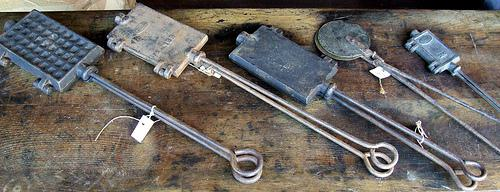
\includegraphics[width=0.175\textwidth]{Images/Comparable/figure1_revisit/original/15749.jpeg}&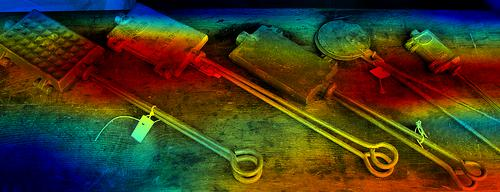
\includegraphics[width=0.175\textwidth]{Images/Comparable/figure1_revisit/raw_att/15749.jpeg}&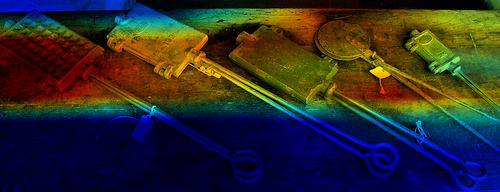
\includegraphics[width=0.175\textwidth]{Images/Comparable/figure1_revisit/shelf_gradcam/15749.jpeg}&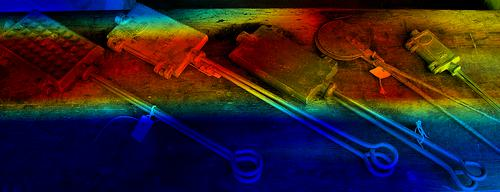
\includegraphics[width=0.175\textwidth]{Images/Comparable/figure1_revisit/gradcam/15749.jpeg}&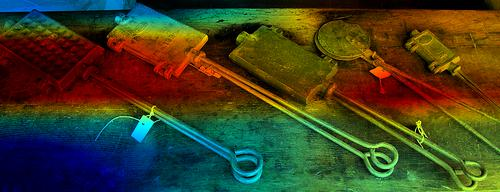
\includegraphics[width=0.175\textwidth]{Images/Comparable/figure1_revisit/shelf_gradcampp/15749.jpeg}&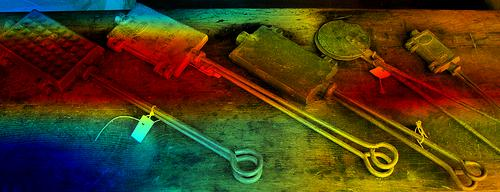
\includegraphics[width=0.175\textwidth]{Images/Comparable/figure1_revisit/gradcampp/15749.jpeg}&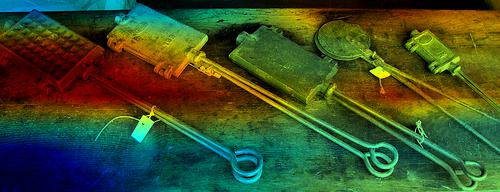
\includegraphics[width=0.175\textwidth]{Images/Comparable/figure1_revisit/scorecam/15749.jpeg}&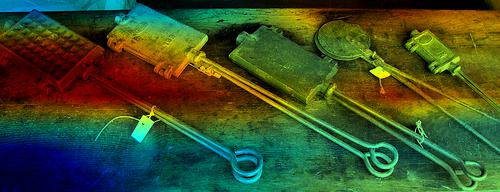
\includegraphics[width=0.175\textwidth]{Images/Comparable/figure1_revisit/scorecam/15749.jpeg}\\

        {\rotatebox{90}{\small Wallaby}}&\multicolumn{1}{c}{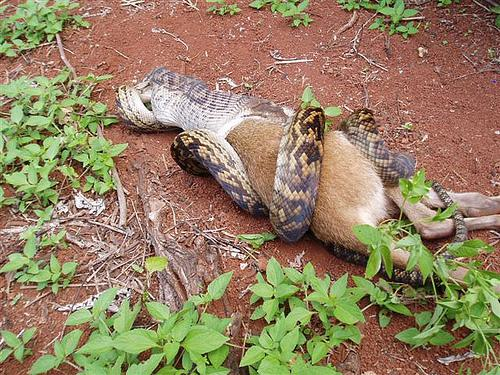
\includegraphics[width=0.175\textwidth]{Images/Comparable/figure1_revisit/original/24263.jpeg}}&\multicolumn{1}{c}{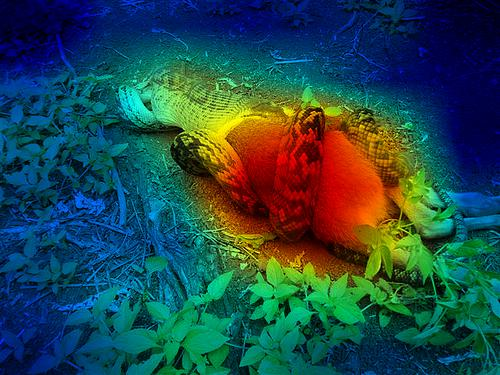
\includegraphics[width=0.175\textwidth]{Images/Comparable/figure1_revisit/raw_att/24263.jpeg}}&\multicolumn{1}{c}{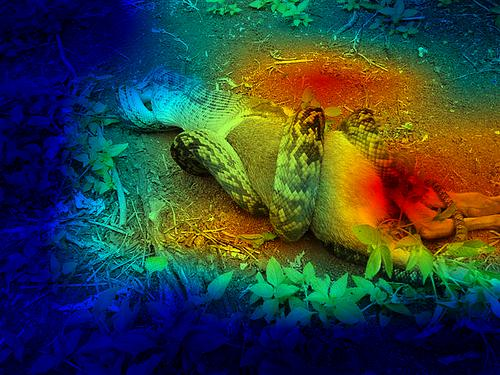
\includegraphics[width=0.175\textwidth]{Images/Comparable/figure1_revisit/shelf_gradcam/24263.jpeg}}&\multicolumn{1}{c}{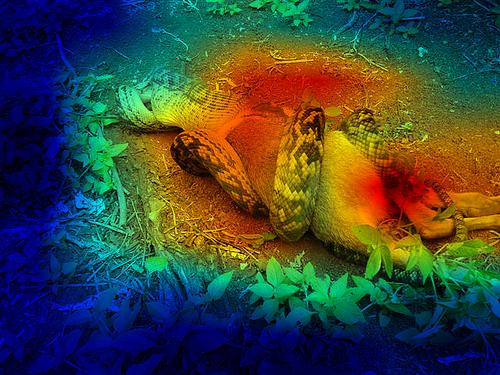
\includegraphics[width=0.175\textwidth]{Images/Comparable/figure1_revisit/gradcam/24263.jpeg}}&\multicolumn{1}{c}{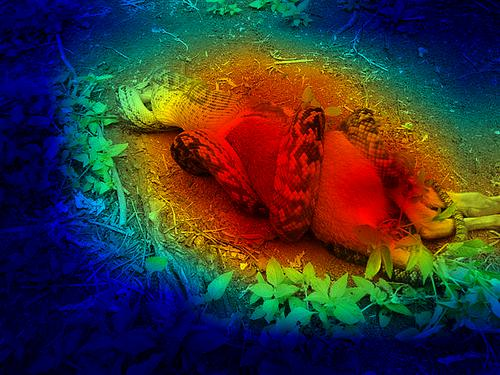
\includegraphics[width=0.175\textwidth]{Images/Comparable/figure1_revisit/shelf_gradcampp/24263.jpeg}}&\multicolumn{1}{c}{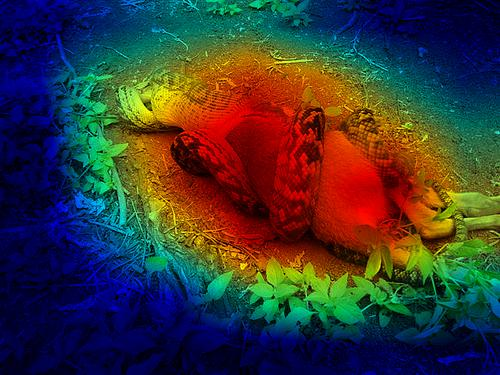
\includegraphics[width=0.175\textwidth]{Images/Comparable/figure1_revisit/gradcampp/24263.jpeg}}&\multicolumn{1}{c}{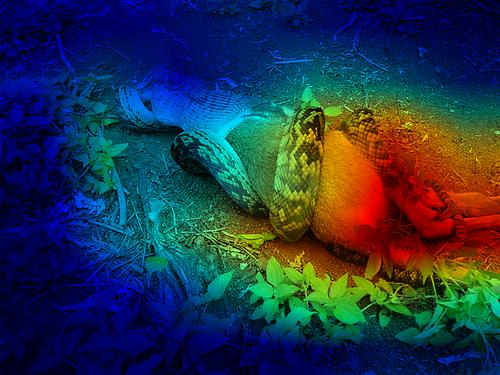
\includegraphics[width=0.175\textwidth]{Images/Comparable/figure1_revisit/scorecam/24263.jpeg}}&\multicolumn{1}{c}{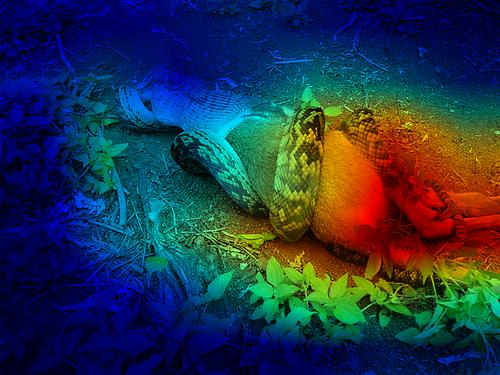
\includegraphics[width=0.175\textwidth]{Images/Comparable/figure1_revisit/scorecam/24263.jpeg}}\\

        {\rotatebox{90}{\small Hoopskirt}}&\multicolumn{1}{c}{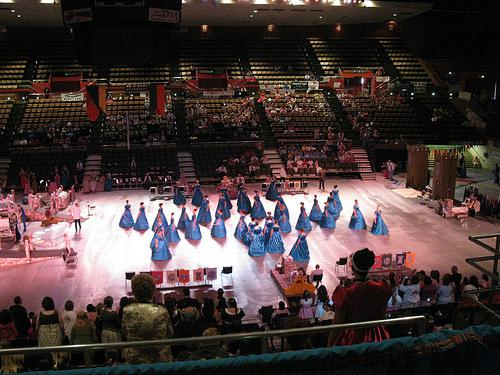
\includegraphics[width=0.175\textwidth]{Images/Comparable/figure1_revisit/original/33003.jpeg}}&\multicolumn{1}{c}{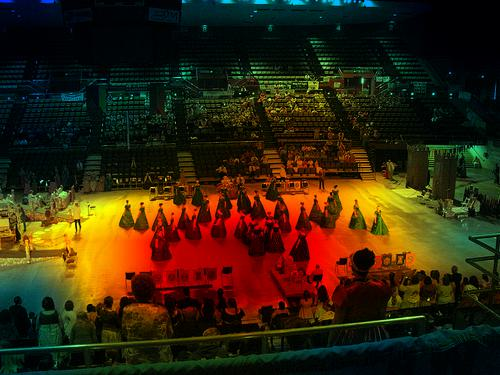
\includegraphics[width=0.175\textwidth]{Images/Comparable/figure1_revisit/raw_att/33003.jpeg}}&\multicolumn{1}{c}{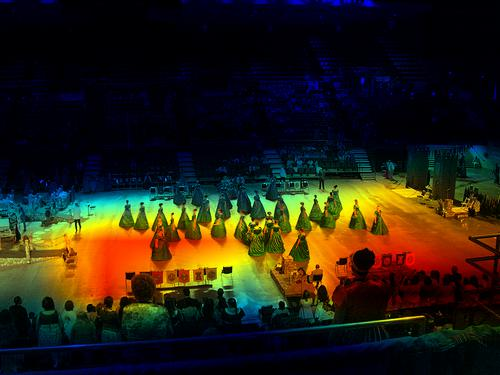
\includegraphics[width=0.175\textwidth]{Images/Comparable/figure1_revisit/shelf_gradcam/33003.jpeg}}&\multicolumn{1}{c}{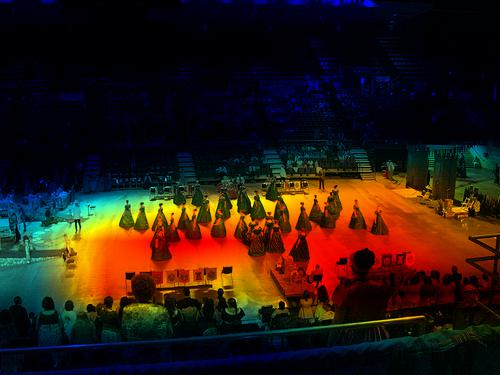
\includegraphics[width=0.175\textwidth]{Images/Comparable/figure1_revisit/gradcam/33003.jpeg}}&\multicolumn{1}{c}{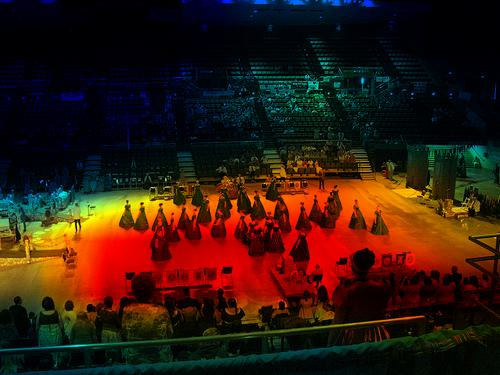
\includegraphics[width=0.175\textwidth]{Images/Comparable/figure1_revisit/shelf_gradcampp/33003.jpeg}}&\multicolumn{1}{c}{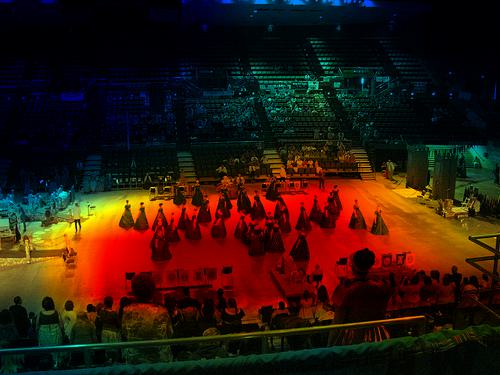
\includegraphics[width=0.175\textwidth]{Images/Comparable/figure1_revisit/gradcampp/33003.jpeg}}&\multicolumn{1}{c}{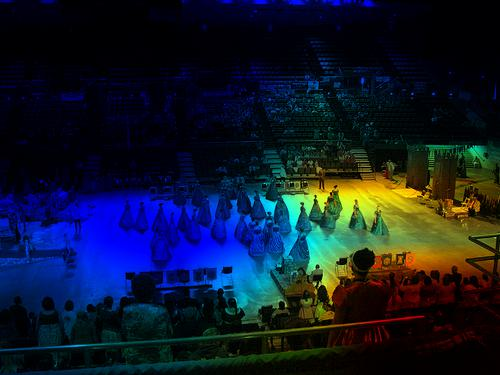
\includegraphics[width=0.175\textwidth]{Images/Comparable/figure1_revisit/scorecam/33003.jpeg}}&\multicolumn{1}{c}{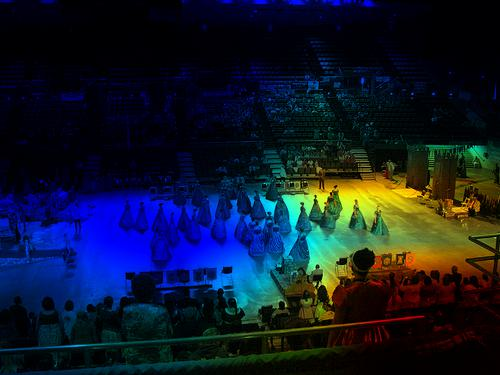
\includegraphics[width=0.175\textwidth]{Images/Comparable/figure1_revisit/scorecam/33003.jpeg}}\\

        {\rotatebox{90}{\small Matchstick}}&\multicolumn{1}{c}{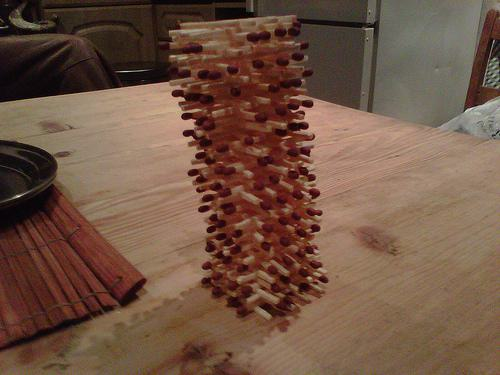
\includegraphics[width=0.175\textwidth]{Images/Comparable/figure1_revisit/original/48096.jpeg}}&\multicolumn{1}{c}{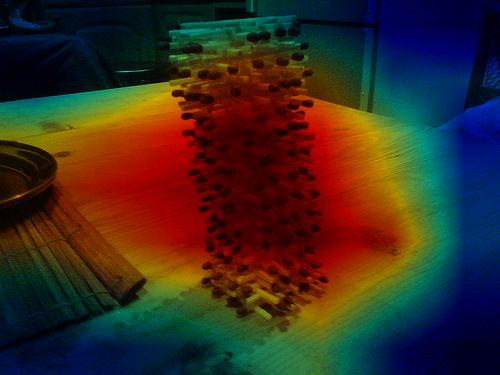
\includegraphics[width=0.175\textwidth]{Images/Comparable/figure1_revisit/raw_att/48096.jpeg}}&\multicolumn{1}{c}{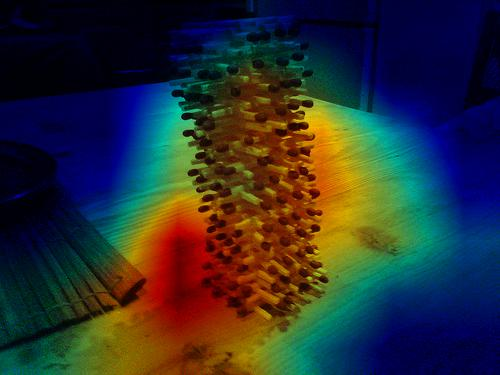
\includegraphics[width=0.175\textwidth]{Images/Comparable/figure1_revisit/shelf_gradcam/48096.jpeg}}&\multicolumn{1}{c}{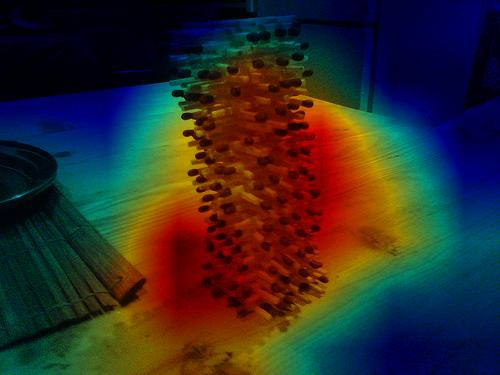
\includegraphics[width=0.175\textwidth]{Images/Comparable/figure1_revisit/gradcam/48096.jpeg}}&\multicolumn{1}{c}{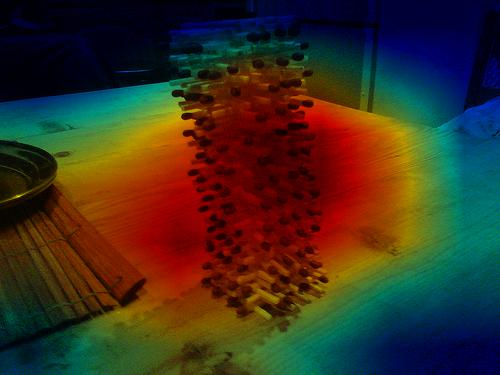
\includegraphics[width=0.175\textwidth]{Images/Comparable/figure1_revisit/shelf_gradcampp/48096.jpeg}}&\multicolumn{1}{c}{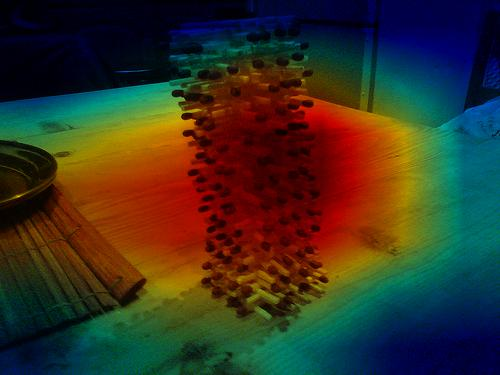
\includegraphics[width=0.175\textwidth]{Images/Comparable/figure1_revisit/gradcampp/48096.jpeg}}&\multicolumn{1}{c}{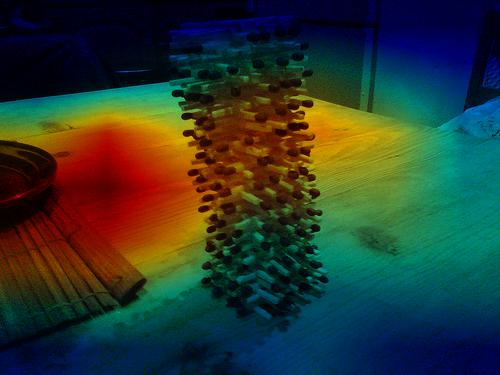
\includegraphics[width=0.175\textwidth]{Images/Comparable/figure1_revisit/scorecam/48096.jpeg}}&\multicolumn{1}{c}{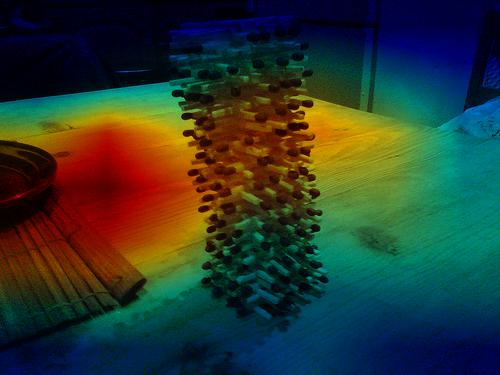
\includegraphics[width=0.175\textwidth]{Images/Comparable/figure1_revisit/scorecam/48096.jpeg}}\\

        {\rotatebox{90}{Sweatshirt}}&\multicolumn{1}{c}{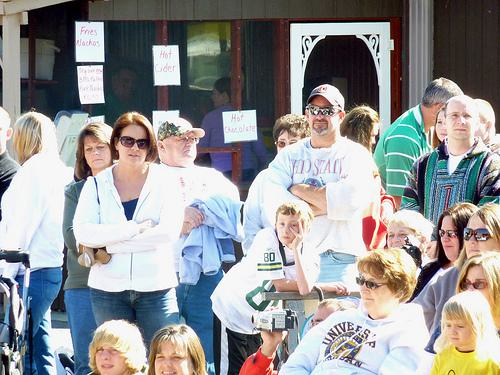
\includegraphics[width=0.175\textwidth]{Images/Comparable/figure1/original/18939.jpeg}}&\multicolumn{1}{c}{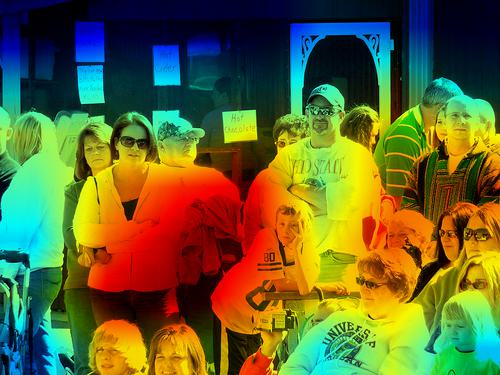
\includegraphics[width=0.175\textwidth]{Images/Comparable/figure1/raw_att/18939.jpeg}}&\multicolumn{1}{c}{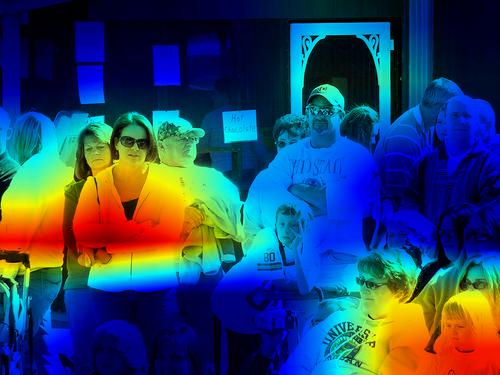
\includegraphics[width=0.175\textwidth]{Images/Comparable/figure1/shelf_gradcam/18939.jpeg}}&\multicolumn{1}{c}{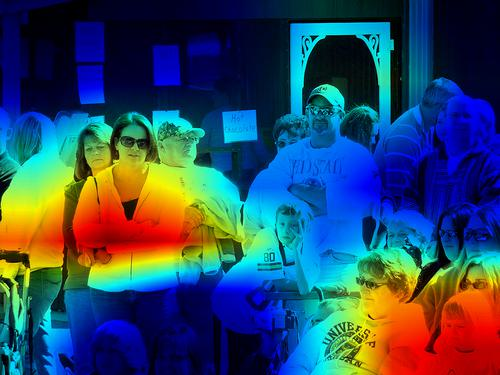
\includegraphics[width=0.175\textwidth]{Images/Comparable/figure1/gradcam/18939.jpeg}}&\multicolumn{1}{c}{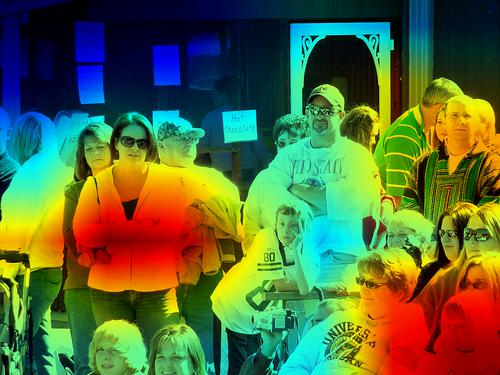
\includegraphics[width=0.175\textwidth]{Images/Comparable/figure1/shelf_gradcampp/18939.jpeg}}&\multicolumn{1}{c}{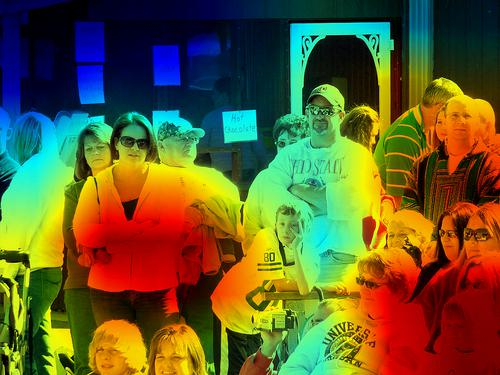
\includegraphics[width=0.175\textwidth]{Images/Comparable/figure1/gradcampp/18939.jpeg}}&\multicolumn{1}{c}{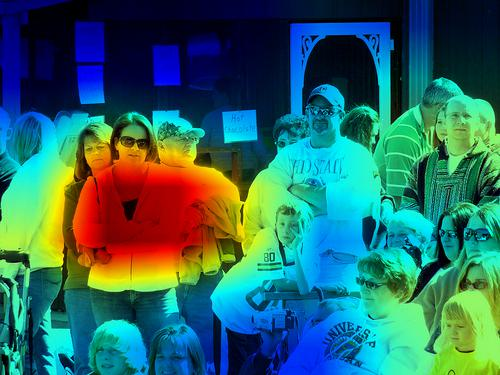
\includegraphics[width=0.175\textwidth]{Images/Comparable/figure1/shelf_scorecam/18939.jpeg}}&\multicolumn{1}{c}{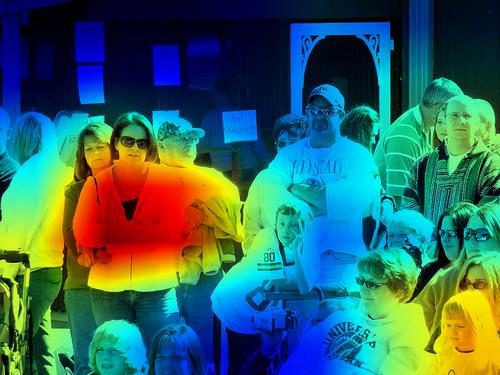
\includegraphics[width=0.175\textwidth]{Images/Comparable/figure1/scorecam/18939.jpeg}}\\

        {\rotatebox{90}{\small CRT screen}}&\multicolumn{1}{c}{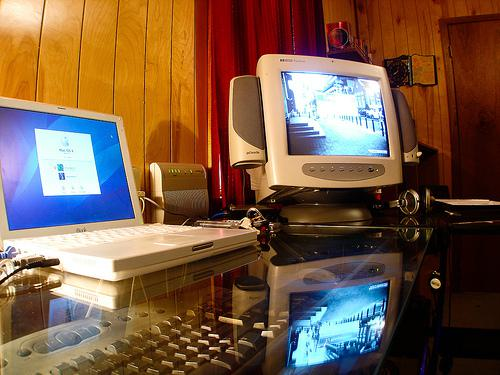
\includegraphics[width=0.175\textwidth]{Images/Comparable/figure1/original/43057.jpeg}}&\multicolumn{1}{c}{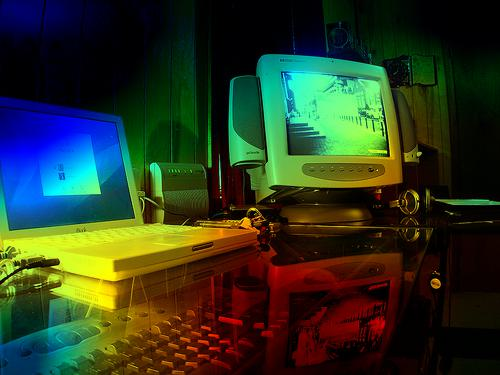
\includegraphics[width=0.175\textwidth]{Images/Comparable/figure1/raw_att/43057.jpeg}}&\multicolumn{1}{c}{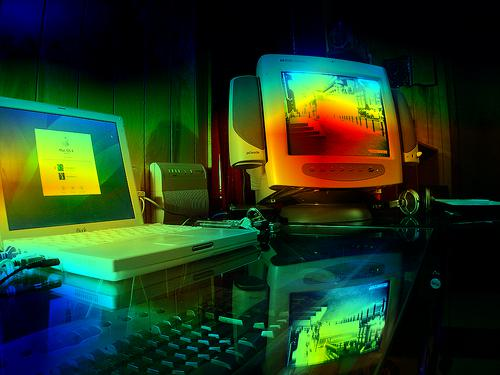
\includegraphics[width=0.175\textwidth]{Images/Comparable/figure1/shelf_gradcam/43057.jpeg}}&\multicolumn{1}{c}{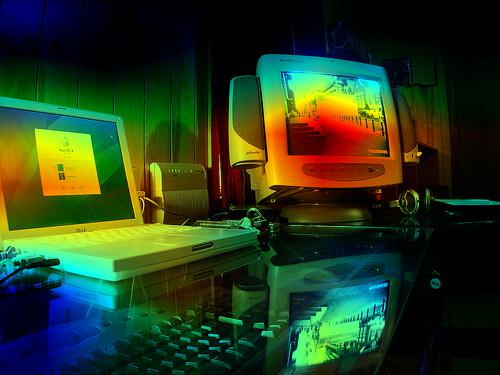
\includegraphics[width=0.175\textwidth]{Images/Comparable/figure1/gradcam/43057.jpeg}}&\multicolumn{1}{c}{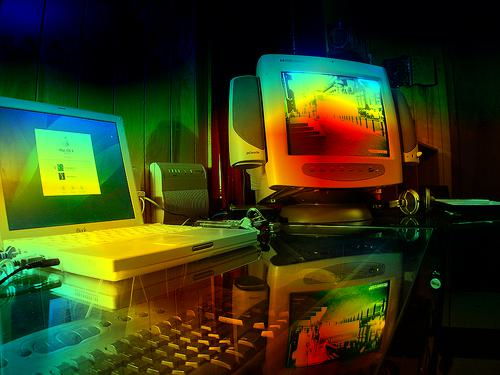
\includegraphics[width=0.175\textwidth]{Images/Comparable/figure1/shelf_gradcampp/43057.jpeg}}&\multicolumn{1}{c}{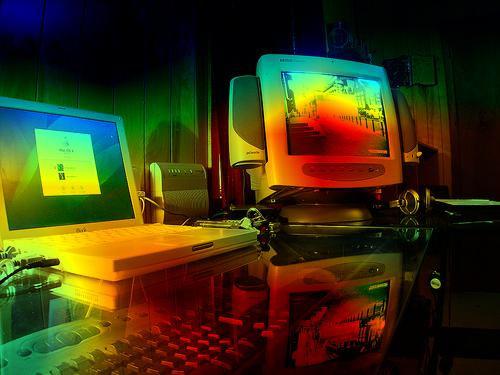
\includegraphics[width=0.175\textwidth]{Images/Comparable/figure1/gradcampp/43057.jpeg}}&\multicolumn{1}{c}{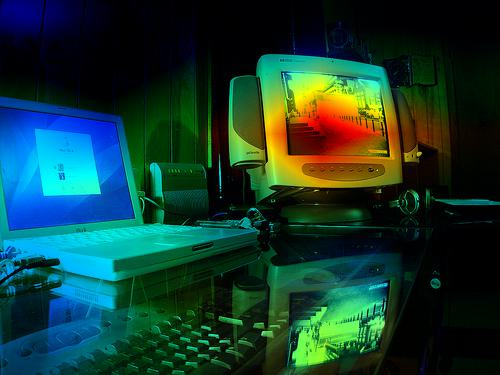
\includegraphics[width=0.175\textwidth]{Images/Comparable/figure1/shelf_scorecam/43057.jpeg}}&\multicolumn{1}{c}{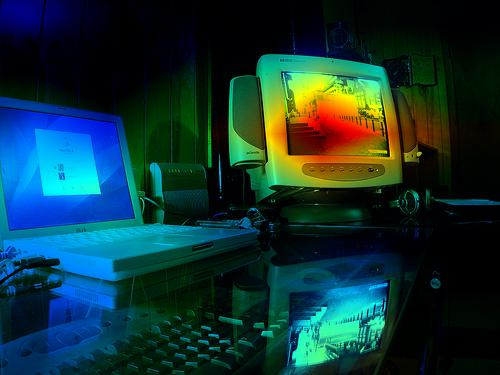
\includegraphics[width=0.175\textwidth]{Images/Comparable/figure1/scorecam/43057.jpeg}}\\ % Checked 
    \end{tabular}
     }
    \caption{Comparison of saliency maps generated by different CAM methods, using GAP or CLS pooling}
    \label{fig:compmethods}
\end{figure*}
%------------------------------------------------------------------------------

%------------------------------------------------------------------------------

\subsection{Qualitative evaluation}
\label{subsec:vinspection}

%% UNDER REVISION
\ronan{We evaluate the quality of saliency maps obtained by  Grad-CAM, Grad-CAM++, and Score-CAM using either [cls] or \gap before the classifier. Moreover, we display the class-agnostic raw attention obtained with [cls], see \autoref{fig:compmethods}.

We observe that raw attention focus on objects of interest in the images.
Moreover the CAM-based techniques have similar saliency maps when using \gap and [cls], as they share the same features maps $F^k_\ell$ and only the weight coefficients $\alpha^c_k$ are modified.
In general, we observe that saliency maps with [cls] tends to cover larger regions of the object or more instances.
The following qualitative experiments show that these changes in saliency maps have a significant impact on the interpretability performances.}

\ronanc{DO WE ADD ATTENTION ONLY ON DATA FROM OTHER DATASETS}

% \begin{figure*}[ht]
    \centering
    \resizebox{\textwidth}{!}{%
    \begin{tabular}{cccccccc}
           \mr{2}{}&\mr{2}{\Th{Original}}&\mc{3}{\Th{First Pass}}&\mc{3}{\Th{Second Pass}}\\
            & &\gap-\Th{GC} & \ours-\Th{GC} & \ours-\Th{RA} &\gap-\Th{GC} & \ours-\Th{GC} & \ours-\Th{RA}\\
           {\rotatebox{90}{\small text}}&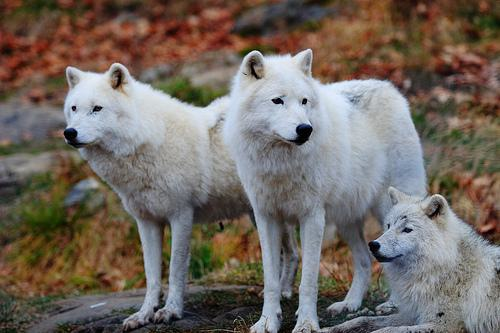
\includegraphics[width=0.1\textwidth]{Images/CLS_Passes/Original/1019.jpeg}&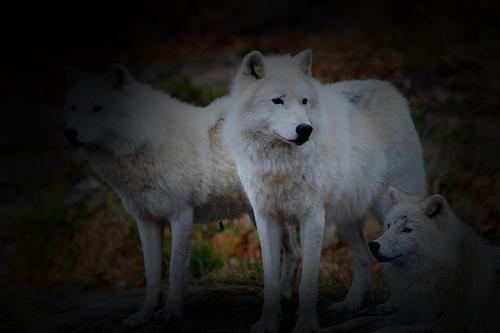
\includegraphics[width=0.1\textwidth]{Images/CLS_Passes/F-Base-CAM/1019.jpeg}&\includegraphics[width=0.1\textwidth]{Images/CLS_Passes/F-Stream-CAM/1019.jpeg}&\includegraphics[width=0.1\textwidth]{Images/CLS_Passes/F-Stream-Raw/1019.jpeg}&\includegraphics[width=0.1\textwidth]{Images/CLS_Passes/S-Base-CAM/1019.jpeg}&\includegraphics[width=0.1\textwidth]{Images/CLS_Passes/S-Stream-CAM/1019.jpeg}&\includegraphics[width=0.1\textwidth]{Images/CLS_Passes/S-Stream-Raw/1019.jpeg}\\

           {\rotatebox{90}{\small text}}&\includegraphics[width=0.1\textwidth]{Images/CLS_Passes/Original/274.jpeg}&\includegraphics[width=0.1\textwidth]{Images/CLS_Passes/F-Base-CAM/274.jpeg}&\includegraphics[width=0.1\textwidth]{Images/CLS_Passes/F-Stream-CAM/274.jpeg}&\includegraphics[width=0.1\textwidth]{Images/CLS_Passes/F-Stream-Raw/274.jpeg}&\includegraphics[width=0.1\textwidth]{Images/CLS_Passes/S-Base-CAM/274.jpeg}&\includegraphics[width=0.1\textwidth]{Images/CLS_Passes/S-Stream-CAM/274.jpeg}&\includegraphics[width=0.1\textwidth]{Images/CLS_Passes/S-Stream-Raw/274.jpeg}\\

           {\rotatebox{90}{\small text}}&\includegraphics[width=0.1\textwidth]{Images/CLS_Passes/Original/963.jpeg}&\includegraphics[width=0.1\textwidth]{Images/CLS_Passes/F-Base-CAM/963.jpeg}&\includegraphics[width=0.1\textwidth]{Images/CLS_Passes/F-Stream-CAM/963.jpeg}&\includegraphics[width=0.1\textwidth]{Images/CLS_Passes/F-Stream-Raw/963.jpeg}&\includegraphics[width=0.1\textwidth]{Images/CLS_Passes/S-Base-CAM/963.jpeg}&\includegraphics[width=0.1\textwidth]{Images/CLS_Passes/S-Stream-CAM/963.jpeg}&\includegraphics[width=0.1\textwidth]{Images/CLS_Passes/S-Stream-Raw/963.jpeg}\\

           {\rotatebox{90}{\small text}}&\includegraphics[width=0.1\textwidth]{Images/CLS_Passes/Original/1944.jpeg}&\includegraphics[width=0.1\textwidth]{Images/CLS_Passes/F-Base-CAM/1944.jpeg}&\includegraphics[width=0.1\textwidth]{Images/CLS_Passes/F-Stream-CAM/1944.jpeg}&\includegraphics[width=0.1\textwidth]{Images/CLS_Passes/F-Stream-Raw/1944.jpeg}&\includegraphics[width=0.1\textwidth]{Images/CLS_Passes/S-Base-CAM/1944.jpeg}&\includegraphics[width=0.1\textwidth]{Images/CLS_Passes/S-Stream-CAM/1944.jpeg}&\includegraphics[width=0.1\textwidth]{Images/CLS_Passes/S-Stream-Raw/1944.jpeg}\\         

          {\rotatebox{90}{\small text}}&\includegraphics[width=0.1\textwidth]{Images/CLS_Passes/Original/711.jpeg}&\includegraphics[width=0.1\textwidth]{Images/CLS_Passes/F-Base-CAM/711.jpeg}&\includegraphics[width=0.1\textwidth]{Images/CLS_Passes/F-Stream-CAM/711.jpeg}&\includegraphics[width=0.1\textwidth]{Images/CLS_Passes/F-Stream-Raw/711.jpeg}&\includegraphics[width=0.1\textwidth]{Images/CLS_Passes/S-Base-CAM/711.jpeg}&\includegraphics[width=0.1\textwidth]{Images/CLS_Passes/S-Stream-CAM/711.jpeg}&\includegraphics[width=0.1\textwidth]{Images/CLS_Passes/S-Stream-Raw/711.jpeg}\\          
    \end{tabular}
    }
    \caption{\emph{Comparison between }}
    \label{fig:com_forwards}
\end{figure*}

%We observe a high degree of similarity between the class-specific explanation maps generated by using both representations. 
%This phenomenon is explained to a great degree by the computation of the weighting coefficient used for CAM methods, as the main factor contributing to these similarities lies within the predictive power of the network, which by itself is affected by the representation used to classify. 
%\autoref{subsec:classification} provides \ronanc{check or clarify the following paragraph maybe} a more concrete explanation of this phenomena. We also observe a contrast between these explanation maps and that produced by attention itself; we note that this representation while covering bigger regions of the image on most instances, presents the most salient points over the object of interest. Ultimately this attention map is used to compute the global representation to classify with.







%///////////////////////////////////old stuff
% We observe that the class-agnostic representation demonstrated by raw-attention, in general covers most of the object of interest of the image,
% We evaluate the quality of the visualizations obtained when using [cls] in comparison to \gap as a representation for classification in \autoref{fig:compmethods}. For this, we compare the class agnostic saliency map obtained by raw attention, and the contrast between Grad-CAM, Grad-CAM++ and ScoreCAM when their computation is carried on using either \gap or [cls].
% In this section, we evaluate the saliency maps generated when we apply the previously mentioned interpretability methods to our approach, in comparison to the baseline models.
% As can be observed on \autoref{fig:compmethods}, the explanation maps generated with the CLS pooling mechanism present a high degree of similarity with those computed using GAP.\\%Conversely on Figure \textit{figure different classes} we observe that our pooling protocol is able to \red{contribution for different classes} when we visualize saliency maps of different categories. Finally, on Figure \textit{contribution towards localization}, we observe that \green{changes on localization given by the application of CLS}.\\
% % We observe that there exists a key factor towards obtaining different saliency maps while following the same interpretability approach.
% % Following our approach and the preservation of the backbone properties, we hypothesize that the small differences obtained for the aforementioned maps are derived from the computation of the weighting coefficient $w_k^c$ previously mentioned in equation \ref{eq:gcam}. Moreover, this coefficient is directly affected by changes on the predictive power for a given network; which on itself can be altered in the same time by the representation of the input image used to classify, be it the GAP features or the [CLS] token. A more detailed explanation of this phenomenon is found in Sections \ref{subsec:interecon} and \ref{subsect:classification}.
% Following our approach and the preservation of the backbone properties, we hypothesize that the small differences observed are derived from the computation of the weighting coefficient $w_k^c$ previously mentioned in equation ~\eq{sal}. Moreover, this coefficient is directly affected by changes on the predictive power for a given network; which on itself is altered at the same time by the representation of the input image used to classify, be it the GAP features or the [CLS] token. A more detailed explanation of this phenomenon is found in \autoref{subsec:interecon} and \autoref{subsect:classification}.
%Sections \ref{subsec:interecon} and \ref{subsect:classification}.

%We hypothesize that while we retain the backbone and classifier layers from the baseline model, the different representations are derived from the computation of the weighting coefficient $w_k^c$ previously mentioned in Equation \ref{eq:gcam}. We note that while we compare explanations provided by the same network and saliency method, the computation of this coefficient is directly affected due changes on the predictive power of the model, which is given by the kind of representation that is used to classify. A more detailed explanation of this phenomenon is found in Sections \ref{subsec:interecon} and \ref{subsect:classification}.

% \begin{figure*}[t]
%     \centering
%     \resizebox{\textwidth}{!}{%
%     \begin{tabular}{ccccccccc}
%         {}&\multirow{2}{*}{Original}&\multirow{2}{*}{Raw Attention}&\multicolumn{2}{c}{Grad-CAM}&\multicolumn{2}{c}{Grad-CAM++}&\multicolumn{1}{c}{Score-CAM}\\
%         {}&{}&{}&GAP&CLS&GAP&CLS&GAP&CLS\\
%         {\rotatebox{90}{\small Car Mirror}}&\multicolumn{1}{c}{\includegraphics[width=0.175\textwidth]{Images/Comparable/figure1/original/351.jpeg}}&\multicolumn{1}{c}{\includegraphics[width=0.175\textwidth]{Images/Comparable/figure1/raw_att/351.jpeg}}&\multicolumn{1}{c}{\includegraphics[width=0.175\textwidth]{Images/Comparable/figure1/shelf_gradcam/351.jpeg}}&\multicolumn{1}{c}{\includegraphics[width=0.175\textwidth]{Images/Comparable/figure1/gradcam/351.jpeg}}&\multicolumn{1}{c}{\includegraphics[width=0.175\textwidth]{Images/Comparable/figure1/shelf_gradcampp/351.jpeg}}&\multicolumn{1}{c}{\includegraphics[width=0.175\textwidth]{Images/Comparable/figure1/gradcampp/351.jpeg}}&\multicolumn{1}{c}{\includegraphics[width=0.175\textwidth]{Images/Comparable/figure1/shelf_scorecam/351.jpeg}}&\multicolumn{1}{c}{\includegraphics[width=0.175\textwidth]{Images/Comparable/figure1/scorecam/351.jpeg}}\\ % Checked for ordering

%         {\rotatebox{90}{\small Sea Cucumber}}&\multicolumn{1}{c}{\includegraphics[width=0.175\textwidth]{Images/Comparable/figure1/original/18852.jpeg}}&\multicolumn{1}{c}{\includegraphics[width=0.175\textwidth]{Images/Comparable/figure1/raw_att/18852.jpeg}}&\multicolumn{1}{c}{\includegraphics[width=0.175\textwidth]{Images/Comparable/figure1/shelf_gradcam/18852.jpeg}}&\multicolumn{1}{c}{\includegraphics[width=0.175\textwidth]{Images/Comparable/figure1/gradcam/18852.jpeg}}&\multicolumn{1}{c}{\includegraphics[width=0.175\textwidth]{Images/Comparable/figure1/shelf_gradcampp/18852.jpeg}}&\multicolumn{1}{c}{\includegraphics[width=0.175\textwidth]{Images/Comparable/figure1/gradcampp/18852.jpeg}}&\multicolumn{1}{c}{\includegraphics[width=0.175\textwidth]{Images/Comparable/figure1/shelf_scorecam/18852.jpeg}}&\multicolumn{1}{c}{\includegraphics[width=0.175\textwidth]{Images/Comparable/figure1/scorecam/18852.jpeg}}\\ %% Checked for ordering

%         {\rotatebox{90}{Sweatshirt}}&\multicolumn{1}{c}{\includegraphics[width=0.175\textwidth]{Images/Comparable/figure1/original/18939.jpeg}}&\multicolumn{1}{c}{\includegraphics[width=0.175\textwidth]{Images/Comparable/figure1/raw_att/18939.jpeg}}&\multicolumn{1}{c}{\includegraphics[width=0.175\textwidth]{Images/Comparable/figure1/shelf_gradcam/18939.jpeg}}&\multicolumn{1}{c}{\includegraphics[width=0.175\textwidth]{Images/Comparable/figure1/gradcam/18939.jpeg}}&\multicolumn{1}{c}{\includegraphics[width=0.175\textwidth]{Images/Comparable/figure1/shelf_gradcampp/18939.jpeg}}&\multicolumn{1}{c}{\includegraphics[width=0.175\textwidth]{Images/Comparable/figure1/gradcampp/18939.jpeg}}&\multicolumn{1}{c}{\includegraphics[width=0.175\textwidth]{Images/Comparable/figure1/shelf_scorecam/18939.jpeg}}&\multicolumn{1}{c}{\includegraphics[width=0.175\textwidth]{Images/Comparable/figure1/scorecam/18939.jpeg}}\\

%         {\rotatebox{90}{Bobsled}}&\multicolumn{1}{c}{\includegraphics[width=0.175\textwidth]{Images/Comparable/figure1/original/20604.jpeg}}&\multicolumn{1}{c}{\includegraphics[width=0.175\textwidth]{Images/Comparable/figure1/raw_att/20604.jpeg}}&\multicolumn{1}{c}{\includegraphics[width=0.175\textwidth]{Images/Comparable/figure1/gradcam/20604.jpeg}}&\multicolumn{1}{c}{\includegraphics[width=0.175\textwidth]{Images/Comparable/figure1/shelf_gradcam/20604.jpeg}}&\multicolumn{1}{c}{\includegraphics[width=0.175\textwidth]{Images/Comparable/figure1/gradcampp/20604.jpeg}}&\multicolumn{1}{c}{\includegraphics[width=0.175\textwidth]{Images/Comparable/figure1/shelf_gradcampp/20604.jpeg}}&\multicolumn{1}{c}{\includegraphics[width=0.175\textwidth]{Images/Comparable/figure1/scorecam/20604.jpeg}}&\multicolumn{1}{c}{\includegraphics[width=0.175\textwidth]{Images/Comparable/figure1/shelf_scorecam/20604.jpeg}}\\%Small differences
             
%         {\rotatebox{90}{Beaver}}&\multicolumn{1}{c}{\includegraphics[width=0.175\textwidth]{Images/Comparable/figure1/original/28492.jpeg}}&\multicolumn{1}{c}{\includegraphics[width=0.175\textwidth]{Images/Comparable/figure1/raw_att/28492.jpeg}}&\multicolumn{1}{c}{\includegraphics[width=0.175\textwidth]{Images/Comparable/figure1/gradcam/28492.jpeg}}&\multicolumn{1}{c}{\includegraphics[width=0.175\textwidth]{Images/Comparable/figure1/shelf_gradcam/28492.jpeg}}&\multicolumn{1}{c}{\includegraphics[width=0.175\textwidth]{Images/Comparable/figure1/gradcampp/28492.jpeg}}&\multicolumn{1}{c}{\includegraphics[width=0.175\textwidth]{Images/Comparable/figure1/shelf_gradcampp/28492.jpeg}}&\multicolumn{1}{c}{\includegraphics[width=0.175\textwidth]{Images/Comparable/figure1/scorecam/28492.jpeg}}&\multicolumn{1}{c}{\includegraphics[width=0.175\textwidth]{Images/Comparable/figure1/shelf_scorecam/28492.jpeg}}\\ % Small differences
              
%         {\rotatebox{90}{\small CRT screen}}&\multicolumn{1}{c}{\includegraphics[width=0.175\textwidth]{Images/Comparable/figure1/original/43057.jpeg}}&\multicolumn{1}{c}{\includegraphics[width=0.175\textwidth]{Images/Comparable/figure1/raw_att/43057.jpeg}}&\multicolumn{1}{c}{\includegraphics[width=0.175\textwidth]{Images/Comparable/figure1/shelf_gradcam/43057.jpeg}}&\multicolumn{1}{c}{\includegraphics[width=0.175\textwidth]{Images/Comparable/figure1/gradcam/43057.jpeg}}&\multicolumn{1}{c}{\includegraphics[width=0.175\textwidth]{Images/Comparable/figure1/shelf_gradcampp/43057.jpeg}}&\multicolumn{1}{c}{\includegraphics[width=0.175\textwidth]{Images/Comparable/figure1/gradcampp/43057.jpeg}}&\multicolumn{1}{c}{\includegraphics[width=0.175\textwidth]{Images/Comparable/figure1/shelf_scorecam/43057.jpeg}}&\multicolumn{1}{c}{\includegraphics[width=0.175\textwidth]{Images/Comparable/figure1/scorecam/43057.jpeg}}\\ % Checked 
%     \end{tabular}
%     }
%     \caption{Comparison of saliency maps generated by different CAM methods, using GAP or CLS pooling}
%     \label{fig:compmethods}
% \end{figure*}
% \subsection{Qualitative Evaluation}
% \label{subsec:vinspection}